In questo capitolo bla bla bla sezione .... \hl{Aggiungere}

\section{Introduzione}
\label{sec:arte_intro}
\paragraph{Optical Character Recognition}
Ad oggi, sempre più libri cartacei, riviste e giornali presenti in biblioteche e archivi storici stanno venendo trasformati in versioni elettroniche che possono essere manipolate da un computer. A questo scopo, nel corso degli anni sono state sviluppate tecnologie di Optical Character Recognition (comunemente abbreviato con OCR) per tradurre le scansioni e immagini di documenti testuali in testo interpretabile e processabile da un computer. Questi sistemi, però, non sono perfetti e possono introdurre errori nel testo. Può accadere, infatti, che durante il processo di scansione alcuni caratteri vengano letti in modo errato, altri vengano aggiunti e altri ancora non riconosciuti. \E, ad esempio, particolarmente probabile che caratteri o sequenze di caratteri graficamente simili come \textit{"li"} e \textit{"n"} vengano scambiati fra di loro\cite{ocr_error_analysis}. La frequenza di tali errori è influenzata da fattori quali la condizione di deterioramento di un documento e la qualità di acquisizione dell'immagine\cite{hartley1999quality}: la presenza di granelli di polvere, caratteri scoloriti, pagine ingiallite o artefatti risultati dalla scansione, ad esempio, influiscono negativamente sulle performance dei sistemi OCR.\\
La presenza di tali errori in corpora acquisiti tramite OCR risulta problematica in quanto rende meno precisi task di Natural Language Processing (NLP) come, ad esempio, l'esecuzione di query \cite{impatto_ocr_1} o il topic modelling\cite{impatto_ocr_2}. Per ovviare a tali problemi, sono state sviluppate varie soluzioni che mirano a minimizzare il quantitativo di errori presenti nel testo estratto. \E\ possibile classificare queste soluzioni nelle seguenti due categorie:
\begin{itemize}
\item \textbf{OCR Pre-processing}: ricadono in questa categoria tutte quelle tecniche che mirano ad ottenere migliori risultati dall'estrazione del testo attraverso il miglioramento dell'input, ovvero delle immagini, che viene usato dai software di OCR. Tali metodi includono, ma non si limitano a, l'uso di migliori tecniche di scansione, la correzione del contrasto nell'immagine\cite{holley2009good} e la rotazione e correzione di deformazioni nell'immagine\cite{bieniecki2007image} (\autoref{fig:art_prep_ex}).
\begin{figure}[H]
\centering
{
\begin{minipage}{0.35\textwidth}
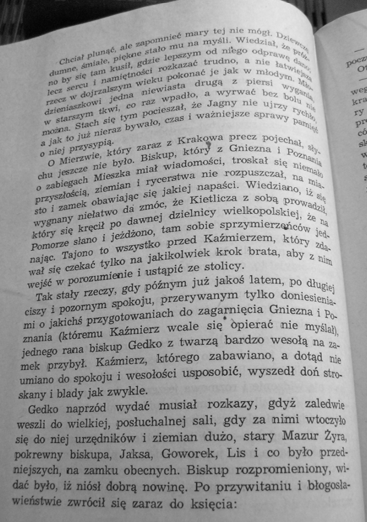
\includegraphics[width=\textwidth]{immagini/stato_arte/prep1}
\end{minipage} 
\begin{minipage}{0.06\textwidth}
\centering
\Large$\rightarrow$
\end{minipage}
\begin{minipage}{0.35\textwidth}
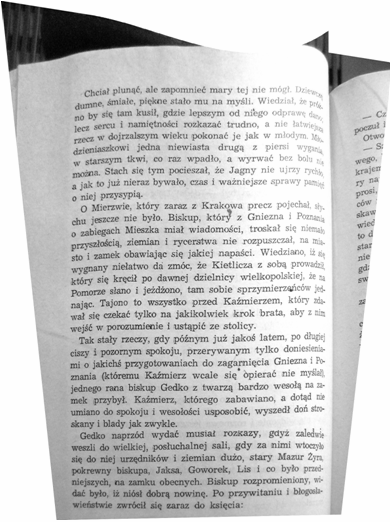
\includegraphics[width=\textwidth]{immagini/stato_arte/prep2}
\end{minipage}
\caption{A sinistra foto di una pagina contenente del testo. A destra, foto della stessa pagina pre-processata per facilitare l'estrazione del testo. Esempio preso da \cite{bieniecki2007image}.}
\label{fig:art_prep_ex}
}
\end{figure}

 
\item \textbf{OCR Post-processing}: ricadono in questa categoria tutte quelle tecniche che mirano ad individuare e correggere gli errori presenti nell'output generato dai vari software di OCR. Essendo l'OCR Post-processing oggetto di questa tesi, sarà approfondito a parte nella \autoref{sec:art_post_post}.
\end{itemize}


OCR pre-processing e post-processing sono spesso usati in congiunzione per ottenere migliori risultati dall'estrazione del testo.

\section{OCR Post-processing}
\label{sec:art_post_post}
In letteratura sono presenti numerosi approcci al problema dell'OCR post-processing, molti dei quali adottano strategie molto differenti. Dato ciò, non è possibile delineare una metodologia generale che ogni approccio segue, ma, in generale, ogni approccio deve:
\begin{enumerate}
\item \textbf{Identificare gli errori} (Error Detection), ovvero delimitare tutte le sezioni contenenti errori nel testo, senza delimitare sezioni corrette. \hl{Espandere?}
\item \textbf{Correggere gli errori} (Error Correction), ovvero ripristinare testo originale nelle sezioni individuate in precedenza. \hl{Espandere?}
\end{enumerate}

Nelle seguenti sottosezioni sono quindi esposti alcuni dei principali approcci per letteratura, raggruppati nelle seguenti categorie di metodologie:
\begin{itemize}
\item Approcci basati su n-grams
\item Approcci basati su NMT
\item Approcci basati su BERT
\item Altri approcci
\end{itemize}

\hl{Controllo che non sia cambiato niente}

\subsection{Approcci basati su n-grams}
Per discutere gli approcci basati sugli n-grams è prima necessario definire i concetti di token, tokenizzazione e n-gram. 

\paragraph{Token}
\E\ riportata la definizione fornita in \cite{tokendef}: "Un token è una stringa di caratteri contigui compresi fra due spazi, o fra uno spazio e un segno di punteggiatura. Sono token anche [numeri] interi, [numeri] reali o numeri contenenti i due punti (ore, ad esempio 2:00). Tutti gli altri simboli sono considerati essi stessi dei token, eccetto gli apostrofi e i punti di domanda attaccati ad una parola (senza spazi), che in molti casi rappresentano acronimi o citazioni."\\
Più informalmente è possibile associare il concetto di token a quello di parola nel linguaggio naturale.

\paragraph{Tokenizzazione}
Data la precedente definizione di token, per tokenizzazione si intende il dividere un testo, una frase, o più in generale una stringa nei token che la compongono. Data quindi una frase $f \in F$, tokenizzare una frase vuol dire applicare una funzione:
\begin{equation}
\textit{Tok}: F \rightarrow T
\end{equation}
dove ogni $t \in T$ è una lista $[t_1,...,t_n]$ in cui ogni $t_i$ è un token appartenente alla frase iniziale.
Più informalmente quindi, la tokenizzazione restituisce le singole parole appartenenti alla frase iniziale. Ad esempio, data la frase $f_{es}$:
\begin{center}
\textit{"Cantami, o Diva, del pelide Achille
l'ira funesta che infiniti addusse
lutti agli Achei"}
\end{center}
la sua versione tokenizzata $\textit{Tok}(f_{es})$ è:
\begin{center}
[\textit{"Cantami"},
\textit{","},
\textit{"o"},
\textit{"Diva"},
\textit{","},
\textit{"del"},
\textit{"pelide"},
\textit{"Achille"},
\textit{"l'"},
\textit{"ira"},
\textit{"funesta"},
\textit{"che"},
\textit{"infiniti"},
\textit{"addusse"},
\textit{"lutti"},
\textit{"agli"},
\textit{"Achei"}]
\end{center}

\paragraph{n-gram} Un n-gram è una sottosequenza contigua di n elementi di una data sequenza \cite{itwiki:ngram}. Gli elementi in questione possono essere fonemi, sillabe, lettere parole ecc. Nel proseguo di questo documento ogni riferimento a n-gram, salvo indicazione contraria, si riferisce a n-gram di token. Gli n-gram trovano ampio uso nel campo del NLP, dove sono usati, ad esempio, per creare modelli linguistici statistici.\\
In seguito è mostrato un esempio di scomposizione di una frase in n-gram di lunghezza 3, detti quindi 3-gram o trigrams. Dato la frase del precedente esempio $f_{es}$, e data la sua scomposizione in token $\textit{Tok}(f_{es})$, i trigrams formati sono i seguenti:
\begin{center}
\textit{["Cantami", ",", "o"]}, \textit{[",", "o", "Diva"]}, \textit{["o", "Diva", ","]}, \textit{["Diva", ",", "del"]}, \textit{[",", "del", "pelide"]}, \textit{["del", "pelide", "Achille"]}, \textit{["pelide", "Achille", "l'"]}, \textit{["Achille", "l'", "ira"]}, \textit{["l'", "ira", "funesta"]}, \textit{["ira", "funesta", "che"]}, \textit{["funesta", "che", "infiniti"]}, \textit{["che", "infiniti", "addusse"]}, \textit{["infiniti", "addusse", "lutti"]}, \textit{["addusse", "lutti", "agli"]}, \textit{["lutti", "agli", "Achei"]}
\end{center}


\paragraph{Approcci basati su n-grams}
\newcommand{\gw}{GW5}
Gli approcci descritti in questa sezione utilizzano modelli linguistici basati su n-gram per individuare e correggere gli errori. Le soluzioni proposte in questa sezione fanno entrambe uso del Google Web 1T 5-gram dataset\cite{google1t}, che da qui in poi verrà riferito come 	\gw. \gw\ è un dataset contenente n-grams in lingua inglese (da unigrams a 5-grams) associati alla loro frequenza osservata su un totale di 1 trilione di parole. Tutti gli n-grams sono stati estratti attraverso il crawling di pagine web. L'enorme scala del database e la metodologia tramite la quale è stato ottenuto comporta che sia possibile estrarre da \gw\ un amplio lessico che può essere affabilmente usato per fare error detection. Per lo stesso motivo, il dataset si presta bene anche all'applicazione in campi con terminologie di nicchia o altamente specifiche.\\
Il primo approccio trattato quello presentato in \cite{ocrG1}. L'approccio è diviso di tre fasi:
\begin{enumerate}
\item Error Detection: sono usati gli unigram in \gw\ per identificare gli errori. Ogni token all'interno del testo da correggere non presente nella lista degli unigram è considerato un errore. \E\ quindi chiaro come questo metodo riesca ad individuare (e quindi correggere) solo i non-word errors, ovvero tutti quelli errori che risultano in parole non presenti in un dato lessico. Non sono trattati da questo approccio i real-word errors, ovvero tutti quelli errori che risultano in una parola presente in un dato lessico. Si pensi ad esempio alla parola \textit{"sale"} interpretata come \textit{"sala"} da un software OCR.

\item Candidate Spelling Generation: per ogni errore si produce una lista di parole candidate per la correzione. Per fare ciò si scompone la parola errata in 2-grams a livello di carattere. Ad esempio, la parola "sangle" è scomposta in "sa", "an", "ng", "gl", "le". Per ognuna delle parole nel lessico di unigram, in seguito, si conta quante occorrenze dei 2-gram della parola da correggere sono contenute. Ad esempio, la parola "single" contiene tre occorrenze ("ng","gl","le"). Le prime 10 parole con più occorrenze dei 2-gram sono considerate i candidati per la correzione.

\item Error Correction: si considera il 5-gram terminante con la parola errata $[t_1,t_2,t_3,t_4,\textit{err}]$. Per ognuno dei candidati $c_i$ è prodotto il 5-gram $[t_1,t_2,t_3,t_4,{c_i}]$: di questi 5-gram prodotti, quello con più occorrenze all'interno di \gw\ contiene la correzione da applicare.
\end{enumerate}

Un approccio simile è esposto in \cite{ocrG2}. A differenza dell'approccio precedente, l'error detection e la generazione dei candidati non usano \gw, ma sono usate altre tecniche che mirano a correggere anche i real-word errors. L'approccio utilizzato per l'error correction invece sfrutta lo stesso principio di \cite{ocrG1}, ma con una logica leggermente più complessa. Il funzionamento è il seguente:
\begin{enumerate}
\item Error Detection e Candidate Generation: per i non-word errors GNU-Aspell\cite{atkinsongnu} è utilizzato per individuare gli errori e proporre i possibili candidati per la correzione. Per i real-word errors invece, sono usati dei confusion-set pre-definiti per individuare i possibili errori e generare i candidati. Un confusion-set non  è altro che un insieme di parole simili che possono essere confuse fra di loro, come \{they'
re, their, there\}. I candidati per un possibile errore sono quindi le parole appartenenti al suo confusion set.

\item Error Correction. Per ogni candidato si considera un intorno di 2 parole, andando così a comporre un 5-gram. Se il 5-gram in cui è presente l'errore nel testo è $[t_1,t_2,\textit{err},t_3,t_4]$, allora per il candidato $c_i$ sarà $[t_1,t_2,c_i,t_3,t_4]$. Il candidato scelto è quello il cui 5-gram compare più volte in \gw. In caso nessun 5-gram compaia nel dataset, il processo si ripete con il 3-gram $[t_2,c_i,t_3]$ e successivamente solo con l'unigram $[c_i]$, ovvero viene scelto il candidato con la maggior frequenza nel corpus.
\end{enumerate}
Gli approcci fin'ora descritti, seppur molto efficaci contro i non-word errors, ma non correggono o sono poco efficaci contro i real-word errors e altri tipi di errori. Si pensi ad esempio a situazioni in cui token viene separato da spazi, o in cui due token sono fusi insieme. Inoltre questi approcci, richiedono un'elevata quantità di dati per funzionare efficacemente (\gw\ occupa 87GiB su disco) , il che non li rende facilmente applicabili.

% Potrei aggiungere cose anche da https://aclanthology.org/H05-1109.pdf
% o da https://ieeexplore.ieee.org/stamp/stamp.jsp?tp=&arnumber=8978061

\subsection{Approcci basati su NMT}




\subsection{Approcci basati su BERT}
\subsection{Altri Approcci}
























